\noindent{\Huge\scshape М}{\LARGE\scshape ировая художественная культура}\\
\rule[0.5\baselineskip]{\textwidth}{1pt}

\vspace{0\baselineskip}


\subsection*{Задание 28.}
    Прочти рассказ Е. Замятина «Десятиминутная драма». Объясни, какую роль в портрете главного героя играют \textit{очки}? На что они указывают, характеризуют ли его социальное положение? Если да, то каким образом? В 1920-е годы были популярны фильмы с Гарольдом Ллойдом, просмотр одного из них может помочь тебе с ответом.
    
    В каких ещё текстах встречается эта же деталь с такой же семантической нагрузкой в портрете персонажа? Для ответа ты можешь обращаться не только к литературе, но и к другим видам искусства.

\subsection*{Задание 29.}
Натюрморт (от фр. \textit{nature morte} — «мёртвая природа») как отдельное направление живописи получил особое распространение в работах голландских живописцев \RimNum{17} века. С тех пор прошли века, многое забылось, и в наши дни слово «натюрморт» зачастую не вызывает никаких ассоциаций, кроме скучных ваз с цветами и фруктами. Однако натюрморты прошлых веков зачастую содержали смерть не только в названии. 
\begin{list}{\asbuk{nnn})}{\usecounter{nnn}\leftmargin=6mm \labelwidth=5mm \topsep=0mm \labelsep=2mm \itemsep=0pt \parsep=0mm \itemindent=-1pt}
\item Внимательно рассмотри картину Антонио Переда «Сон рыцаря», датируемую серединой \RimNum{17} века; её ты сможешь найти в Интернете.  Определи, к какому жанру относится присутствующий на ней натюрморт (см. фрагмент на Рис.~\ref{son}, стр.~\pageref{son}).
    
\begin{figure}
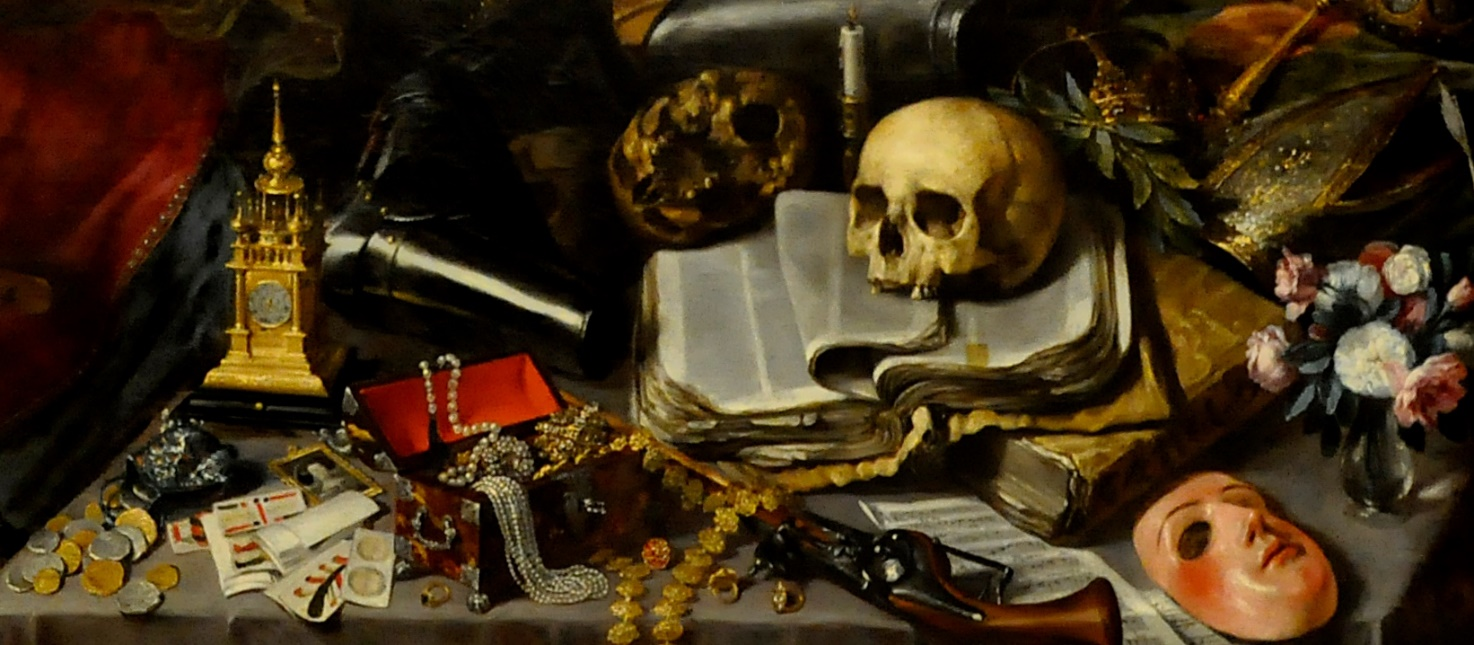
\includegraphics[width=\textwidth]{images/image1-17.jpeg}
\caption{\label{son}А.\,Переда, «Сон рыцаря», фрагмент}
\end{figure}
    
\hspace*{5mm}Известно, что работавшие в этом жанре живописцы придавали большое значение символике изображаемых предметов, за каждым из которых был закреплен аллегорический смысл. Зачастую символы на картине складывались в цельное высказывание, обычно моралистического или нравоучительного характера. 

\iffalse\begin{center}
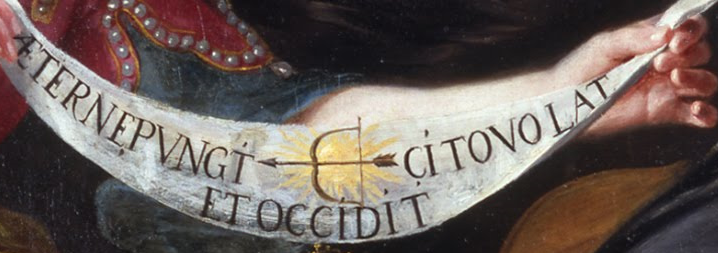
\includegraphics[width=0.5\textwidth]{images/image2-19.png}
\end{center}\fi
\begin{minipage}{0.94\textwidth}    
\setlength{\intextsep}{0.2pt} 
\setlength\columnsep{7.2pt}
\begin{wrapfigure}{r}{7.1cm}
{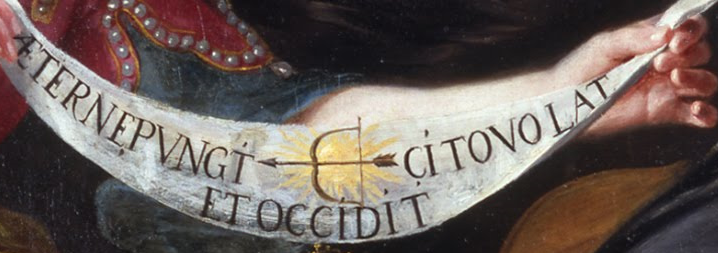
\includegraphics[width=7.04cm]{images/image2-19.png}}
\caption{\label{son-kusok}Фрагмент катины А.\,Переда, «Сон рыцаря»}
\end{wrapfigure}
\item Найди на упомянутом натюрморте как можно больше изображений различных объектов, которые, с твоей точки зрения, являются символами. Свой выбор обоснуй. Что обозначают эти символы и их композиция? Как связана эта композиция с латинской фразой в центре картины (см. Рис.~\ref{son-kusok})? 

\item Приведи в пример ещё пять картин подобного жанра (их изображения найди в интернете), выполненных в различные эпохи — от \RimNum{17} до \RimNum{20} века. Предметы каких типов присутствуют на картинах каждой эпохи? Объясни символическое значение этих предметов и предположи, с чем связано их устойчивое присутствие.\end{minipage}
\end{list}\vspace{\parsep}

О различных жанрах голландского натюрморта ты можешь прочесть в книге Ю.А. Тарасова «Голландский натюрморт \RimNum{17} века», а узнать о концепции символа в живописи, а также о значениях наиболее распространённых символов из книги Ю.Н. Звездиной «Эмблематика в мире старинного натюрморта».

\subsection*{Задание 30.}
    Прочитай статью Зинаиды Гиппиус «Положение литературной критики» (под псевдонимом Антон Крайний) и ответь на вопросы: а) почему в статье поднимается вопрос о роли литературной критики? С чем это связано? б) какие цели у данной статьи? в) можно ли сказать, что данная литературно-критическая статья обладает чертами публицистики? Если да, то почему?
    
    В качестве теоретической базы можешь использовать материал из книги История русской литературной критики: советская и постсоветская эпохи / под ред. Е. Добренко, Г. Тиханова. М.: Новое литературное обозрение.  С. 347–350. 
